\documentclass{article}
\usepackage[a4paper]{geometry}
\usepackage{amsfonts}
\usepackage{alltt}
\usepackage{amsmath,amssymb}        % Mathpack für Formeln jeder Art
\usepackage[parfill]{parskip}       % Autoamtisch Newline, wenn Zeilenumbruch im Quelltext.
\usepackage[utf8]{inputenc}         % UTF8 Zeichensatz. 
\usepackage{xstring}				% Gebraucht für Circuitikz
\usepackage{tikz}                   % Wichtig für Zeichnungen aller Art
\input{kvmacros}                    % Kv Diagramme
\usepackage[siunitx]{circuitikz}    % Diagramme und Schaltungen
\usepackage{pgffor}
\usepackage{fancyhdr}
\usepackage{array}
\usepackage{fullpage}
\usetikzlibrary{arrows,automata}


\tikzstyle{help lines}=[blue!50,very thin]
\tikzstyle{help lines}+=[dashed]
\tikzstyle{Kreis}= [circle,draw]


\title{RS - Übung 9}
\author{Arne Beer (MN 6489196), \\
Rafael Epplee (MN 6269560)}



\begin{document}
\maketitle

\section*{Aufgabe 1}

	\subsection*{a)}
		
		Der Hauptautomat ist ein einfacher Moore Automat mit 4 Zuständen und lediglich einem Enable. Vom Zählerautomaten geht eine Leitung zum Hauptautomaten, welche übermittelt, wann der Zähler wieder bei 0 angelangt. Dies trifft ein, wenn der Zähler einmal durchgelaufen ist oder ein Reset durchgeführt wurde. Der Zustand definiert hingegen wieder 2 Werte und zwar $y_0$ und $y_1$. $Z_0$, also die Grünphase, legt z.B. $y$ als Ausgangswert fest. 

		Der Zählerautomat ist ein 16-bit Zähler mit Reset sodass hier durch einen Ablauf von 35000 Takten bei einer 1 KHz-Taktung eine ausreichende Verzögerung für die Dauer einer Rotphase erzeugt wird. Vom Hauptautomaten geht eine Leitung zum Zählerautomaten, die den Reset bestimmt, in unserem Fall die Werte $y_0$ und $y_1$. So wird immer in Reset an der gewünschten Stelle durchgeführt.

		In der Aufgabenstellung wird gesagt, dass beide Automamten mit dem selben Takt laufen. Alternativ könnte, man jedoch einstellen, dass der Hauptautomat nicht auf einen Enable reagiert, sondern einfach den Enable des Zählerautomaten als Clock interpretiert. Das hat den Vorteil, dass der Hauptautomat nicht tausende Male schaltet, sondern nur, wenn es notwendig ist. 
		
		

	\subsection*{b)}



	\subsection*{c)}



	\subsection*{d)}

		Der Hauptautomat hat die vier Zustände $Z_0$ - $Z_3$, welche die für die Ampeln notwendige Steuerung als Ausgänge haben. Außerdem werden für jeden Zustand die Werte $y_0$ und $y_1$ definiert, die dem Zählerautomaten angeben, an welcher Stelle ein Reset durchgeführt werden soll. Der Zähler ist demzufolge ein 16-Bit Addierer mit Reset, da mindestens 35000 Zustände dargestellt werden müssen. Vom Zähler aus geht eine Leitung zum Hauptautomaten, der entweder den Enable oder die Clock des Hauptautomaten darstellt. Die Clock wäre eine vorteilhaftere Wahl, da in diesem Falle der Hauptautomat nicht mit 1 KHz getaktet würde. \\

		$\overline{y_1} \overline{y_0}$ stellt hier die Bedingung für einen Reset bei 30000 dar.\\
		$\overline{y_1}y_0$ stellt hier die Bedingung für einen Reset bei 3000 dar.\\
		$y_1\overline{y_0}$ stellt hier die Bedingung für einen Reset bei 35000 dar.\\
		$y_1y_0$ stellt hier die Bedingung für einen Reset bei 5000 dar.\\

		
		Mit dem folgenden Diagramm wird ein Automat dargestellt, der mit dem selben Takt arbeitet, wie der Zählerautomat und lediglich durch einen Enable weiterschaltet. 
		Wenn man den Enable des Zählerautomaten nun jedoch als Takt verwendet, würden die Schleifen an den einzelnen Zuständen und die Bedingung e für den nächsten Zustand entfallen. 


		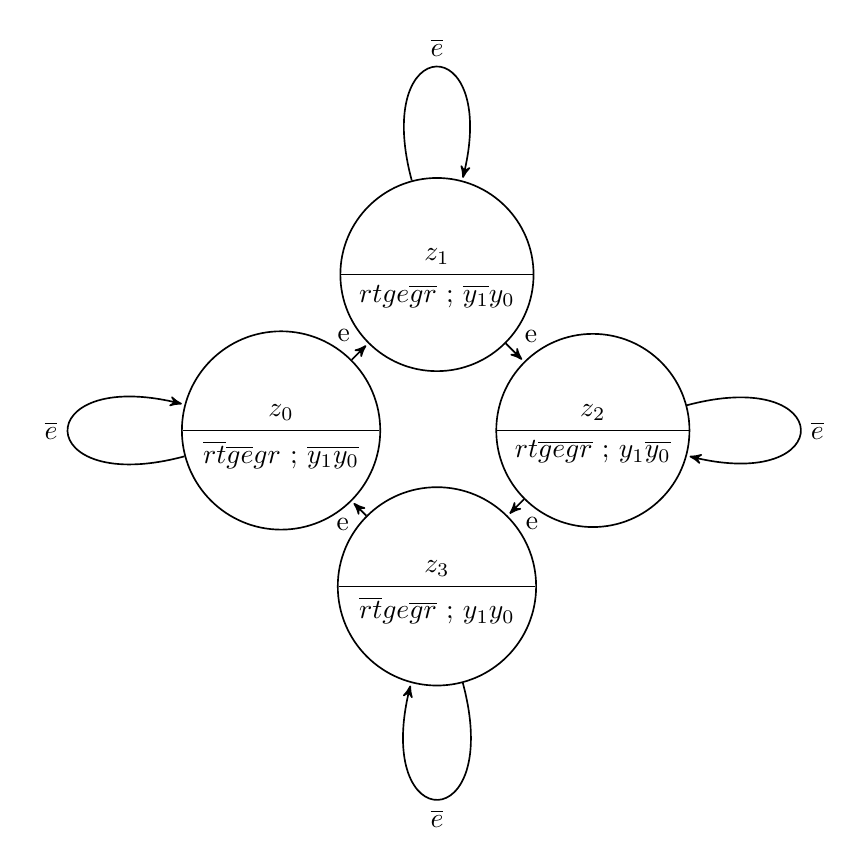
\begin{tikzpicture}[->,>=stealth',shorten >=1pt,auto,node distance=2.8cm,
	                    semithick]
	  	\tikzstyle{every state}=[circle split, draw]

		  \node[state]		  (A)                    {$z_0$\nodepart{lower} $\overline{rt}\overline{ge}gr$ ; $\overline{y_1} \overline{y_0}$ };
		  \node[state]         (B) [above right of=A] {$z_1$\nodepart{lower} $rtge\overline{gr}$ ; $\overline{y_1}y_0$ };
		  \node[state]         (C) [below right of=B] {$z_2$\nodepart{lower}$rt\overline{ge}\overline{gr}$ ; $y_1\overline{y_0}$};
		  \node[state]         (D) [below right of=A] {$z_3$\nodepart{lower}$\overline{rt}ge\overline{gr}$ ; $y_1y_0$};


		  \path (A) edge              node {e} (B)
		            edge [loop left]  node {$\overline{e}$} (A)
		        (B) edge [loop above] node {$\overline{e}$} (B)
		            edge              node {e} (C)
		        (C) edge              node {e} (D)
		            edge [loop right] node {$\overline{e}$} (C)
		        (D) edge [loop below] node {$\overline{e}$} (D)
		            edge              node {e} (A)
		;
		\end{tikzpicture}


\section*{Aufgabe 2}

	\subsection*{a)}

		\begin{tabular}{|c|c c|c c|c c|c c|} \hline
		$Z_x$ &$z_0$ & $z_1$ & ${z^+}_0$ & ${z^+}_1$ & $x_0$ & $x_1$ & $y_0$ & $y_1$\\ \hline
		$Z_0$&0&0&0&0&1&*&0&1 \\
		$Z_0$&0&0&0&1&0&*&0&1 \\
		$Z_1$&0&1&0&1&0&*&1&0 \\
		$Z_1$&0&1&1&0&1&1&1&0 \\
		$Z_1$&0&1&1&1&1&0&1&0 \\
		$Z_2$&1&0&1&0&*&1&1&0 \\
		$Z_2$&1&0&0&1&0&0&1&0 \\
		$Z_2$&1&0&0&0&1&0&1&0 \\
		$Z_3$&1&1&1&1&1&*&1&1 \\
		$Z_3$&1&1&1&0&0&*&1&1 \\\hline

		\end{tabular}
 
 \		


	$\delta(Z_2, \overline{x_1}x_0)=\delta(Z_0, x_0)=Z_0$\\
	$\delta(Z_0,\overline{x_0})= \delta(Z_1,\overline{x_0})=\delta(Z_2,\overline{x_0}\overline{x_1})=Z_1$ \\
	$\delta(Z_1,x_1 x_0)=\delta(Z_2,x_1)=\delta(Z_3,\overline{x_0})=Z_2$\\
	$\delta(Z_1, \overline{x_1}x_0)=\delta(Z_3,x_0)=Z_3$\\

	\subsection*{b)}



	\subsection*{c)}

		Der Automat ist vollständig und wiederspruchsfrei. 

		$Z_0: x_0\wedge \overline{x_0}=0$ \\
		$Z_1: \overline{x_0} \wedge x_1x_0 \wedge \overline{x_1}x_0 =0 $ \\
		$Z_2: x_1\wedge\overline{x_1}x_0\wedge \overline{x_1}\overline{x_0}=0$ \\
		$Z_3: x_0\wedge \overline{x_0}=0$

		$Z_0: x_0\vee \overline{x_0}=1$ \\
		$Z_1: \overline{x_0} \vee x_1x_0 \vee \overline{x_1}x_0 =1 $ \\
		$Z_2: x_1\vee\overline{x_1}x_0\vee \overline{x_1}\overline{x_0}=1$ \\
		$Z_3: x_0\vee \overline{x_0}=1$

\section*{Aufgabe 3}

	\subsection*{a)}
	\subsection*{b)}
	\subsection*{c)}



\end{document}